\documentclass[14pt]{extarticle}
\usepackage{amsmath}
\usepackage{amssymb}
\usepackage{graphicx}
\graphicspath{ {../chap11/} }
\usepackage[top=1in, bottom=0.75in, left=0.75in, right=0.75in]{geometry}
\newcommand*{\Scale}[2][4]{\scalebox{#1}{\ensuremath{#2}}}%
\usepackage{hyperref}
\usepackage[most]{tcolorbox}
\definecolor{bg}{RGB}{255,249,227}


\begin{document}

\section*{Math 208 Discussion Outline for 12/08/2020}


\subsection{Homework and other due dates}
\begin{itemize}
\item Section 10.7 due 12/08
\item Section 11.1 due 12/11
\end{itemize}

\subsection{Questions?}
\begin{itemize}
	\item Section 10.3-57: Not using the quotient rule, how might you find the derivative of $1/x$?
\end{itemize}

\subsection{Goals}
\begin{itemize}
	\item Cover Section 11.1: First Derivative and Graphs
	\item Create and interpret a sign chart
	\item Draw a graph using the sign chart
\end{itemize}

\subsection{Section 11.1: First Derivative and Graphs}
\subsubsection*{Understanding the graph and f'}
Local minima and maxima occur when $f'(c) = 0$. But not always. The function must pass from
\begin{itemize}
	\item increasing to decreasing ($f'+++$ to $f'---$) for a \textbf{maximum}
	\item decreasing to increasing ($f'---$ to $f'+++$) for a \textbf{minimum}
\end{itemize}
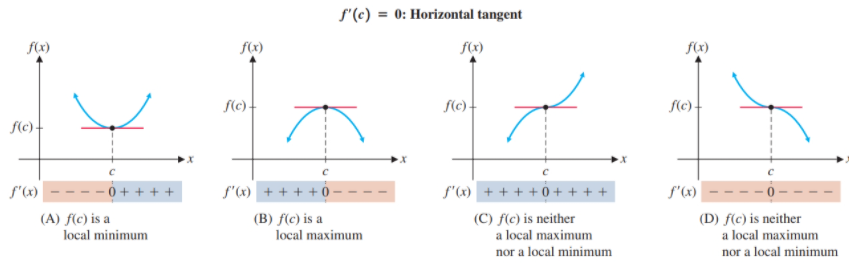
\includegraphics[width=1.0\linewidth]{11-1-1}
\\
\\
And sometimes when f'(c) is not defined. $f'$ is not defined when the slope is infinite or the function is not "smooth".
\\
\\
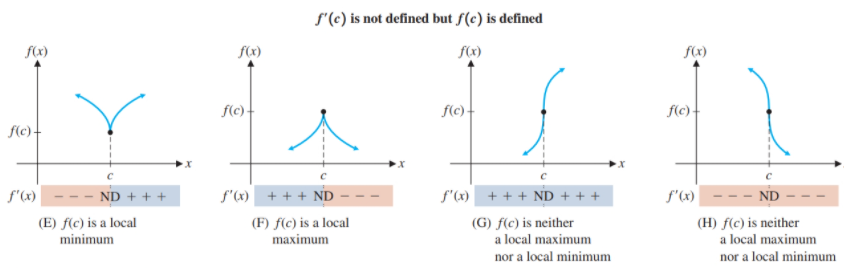
\includegraphics[width=1.0\linewidth]{11-1-2}
\\
Notice the colored bars under the graphs. These \textbf{sign charts} indicate the behavior of $f'$ in those intervals of the graph.

\subsubsection*{Examples}
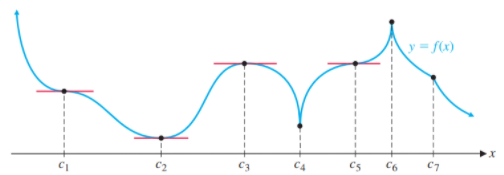
\includegraphics[width=1.0\linewidth]{11-1-3}
\vspace{1cm}
\\
For the graph above, do the following: (similar to problems 9-17)
\begin{enumerate}
	\item Construct a sign chart.
	\item Identify local maxima and minima.
\end{enumerate}

\cleardoublepage

\begin{flalign*}
	&\text{(35) } f(x) = -2x^2 -16x -25 & \tag{Create and interpret sign chart}
\end{flalign*}
\begin{align*}
	f'(x)&= -4x-16 = 0 \tag{When does f' equal 0?}\\
	4x &= -16 \\
	x &= -4 \tag{Only 1 root} \\\\
	f'(-10) &= 40 - 16 > 0 \\
	f'(0) &= -16 <0 \\\\
	\begin{bmatrix}
		&-4& \\
		+++&0&---
	\end{bmatrix}
\end{align*}
Therefore $f(-4)$ is a maximum.
\vspace{1cm}
\begin{flalign*}
	&\text{(43) } f(x) = x^4 +4x^3 +30 & \tag{Create and interpret sign chart}
\end{flalign*}
\begin{align*}
	f'(x)&=4x^3 + 12x^2 = 0 \tag{When does f' equal 0?}\\
	0 &= 4x^2(x + 3) \\
	x &= -3 \tag{Root} \\
	x &= 0 \tag{Double root} \\\\
	f'(-10) &= -4000 + 1200 < 0 \\
	f'(-1) &= -4 + 12 > 0 \\
	f'(1) &= 4 + 12 > 0 \\\\
	\begin{bmatrix}
		&-3& &0& \\
		---&0&+++&0&+++
	\end{bmatrix}
\end{align*}
Therefore $f(-3)$ is a minimum but $f(0)$ is not an extrema. Now draw the graph.

\subsubsection*{Homework}
9-17 all, 33, 37, 39, 41, 51, 53, 55




\cleardoublepage

\end{document}
